%!TEX program = xelatex
\documentclass[12pt,a4paper]{report}

\usepackage{amssymb}
\usepackage{amsmath}
\usepackage{amsthm}
\usepackage{mathtools}
\usepackage{clrscode3e}
\usepackage{graphicx}
\usepackage{listings}
\usepackage{subfig}
\usepackage{listing}
\usepackage{enumitem}
\usepackage{url}
\usepackage{tcolorbox}
\usepackage{tikz}
\usepackage{tabularx}
\lstset{basicstyle=\ttfamily}
\usetikzlibrary{calc,shapes.multipart,chains,arrows}


\usepackage{fontspec}
%\setmainfont{Gill Sans MT}
%\setmainfont{Helvetica}

\pagestyle{plain}

\linespread{1.3}
\textwidth=16cm \textheight=23cm \voffset=-1cm \hoffset=-1.5cm

\theoremstyle{definition}
\newtheorem{problem}{\textbf{Problem}}
\newtheorem{example}{Example}


\theoremstyle{definition}
\newtheorem{definition}{Definition}

\makeatother
\newcommand{\fontitem}{\Large}
\newcommand{\fontitemi}{\normalsize}
\newcommand{\fontitemii}{\normalsize}

\DeclarePairedDelimiter\ceil{\lceil}{\rceil}
\DeclarePairedDelimiter\floor{\lfloor}{\rfloor}

\def\headline#1{\hbox to \hsize{\hrulefill\quad\lower.3em\hbox{#1}\quad\hrulefill}}
\def\headline#1{\hbox to \hsize{\hrulefill\quad\lower.3em\hbox{#1}\quad\hrulefill}}

\begin{document}

\begin{center}
\textbf{\Large Data Structure and Algorithm, Spring 2018\\}
\textbf{\Large Homework \#1\\} 
\vspace{5pt}
\textbf{Release: Tuesday, March 13, 2018}\\
\textbf{Due: Tuesday, March 29, 2018}\\
TA E-mail: dsa1@csie.ntu.edu.tw\\

\textbf{
\end{center}

\vspace{5pt}

\begin{center}
\textbf{\large Non-Programming problems}
\end{center}
\vspace{10pt}

\begin{problem} Stack/Queue

    You have learned in class that stack is a FILO/LIFO data structure and that queue is a FIFO/LILO data structure.
    Please design an algorithm(pseudo code) under the following scenarios. They are all independent.
    You can assume that all data structure mentioned below have infinite capacity and all operations are valid.
    That is, no \texttt{Pop()} will be called on an empty stack and no \texttt{DeQueue()} will be called on an empty queue.
\begin{enumerate}[label=\alph*.]
    \item Please use $2$ queues and $O(1)$ extra space to simulate a stack. That is, please implement \texttt{Pop()}, \texttt{Push()} and \texttt{IsEmpty()} of a stack.
    \item Please use $2$ stacks and $O(1)$ extra space to simulate a queue. That is, please implement \texttt{DeQueue()}, \texttt{EnQueue()} and \texttt{IsEmpty()} of a queue.
\end{enumerate}
    You are given a stack $S$ and a queue $Q$. They both have infinite capacity, and they both store positive integers. The numbers of elements of $S$ and $Q$ will both be not greater than $n$. Please describe a procedure to determine whether there exists common element between $S$ and $Q$ in the following scenarios. If there exists, please output arbitrarily one of the common elements. If not, please output $0$.  The scenarios are independent, and you can answer them in any order.
\begin{enumerate}[label=\alph*.]
    \setcounter{enumi}{2}
\item Guaranteed that the elements in $S$, from bottom to top, are strictly increasing, and the elements in $Q$, from rear to front, are also strictly \textbf{increasing}. In $O(n)$ time, $O(1)$ extra space.
\item Guaranteed that the elements in $S$, from bottom to top, are strictly increasing, while the elements in $Q$, from rear to front, are strictly \textbf{decreasing}. In $O(n)$ time, $O(1)$ extra space.
\end{enumerate}
\end{problem}
\newpage

\begin{problem}Complexity

In this part, if you would like to use any theorem which is not mentioned in class, please prove it in advance.
\begin{center}
$\lg(n) = \log_2(n)$, $\ln(n) = \log_e(n)$, $\log(n) = \log_{10}(n)$
\end{center}

\begin{enumerate}[label=\arabic*.]
\item Please rank the following functions by the order of growth. No proof or extra statement is needed.
    \begin{center}$4^n, 8^n, n^2, n^n, n\lg n, e^{\ln(n)}, 2^{\sqrt{\lg n}}$\end{center}
\item Prove that $\log(n!) = O(n\lg n)$
\item Prove or disprove the following statements. You should provide a formal proof or a counterexample for each statement. Please note that in the following statements, $f(n), g(n), i(n), j(n)$ are non-negative, monotonically increasing functions. That is, the union of ranges of these functions is a subset of $\mathbb{R}^+\cup\{0\}$, and $n_1>n_2 \implies f(n_1)\geq f(n_2), g(n_1)\geq g(n_2), i(n_1)\geq i(n_2), j(n_1)\geq j(n_2)$.
    \begin{enumerate}[label=\alph*.]
    \item $100n^2+300n = O(n^2)$.
    \item If $f(n) = O(i(n))$, $g(n) = O(j(n))$, then $f(n) - g(n) = O(i(n) - j(n))$.
    \item If $f(n) = O(g(n))$, then $f^2 = O(g^2)$.
    \item If $f(n) = \Omega(i(n))$, $g(n) = \Omega(j(n))$, then $f(n) + g(n) = \Omega(i(n) + j(n))$
    \item If $f(n) = O(g(n))$, then $2^{f(n)} = O(2^{g(n)})$
    \item If $2^{f(n)} = O(2^{g(n)})$, then $f(n) = O(g(n))$
    \item $f(n) + g(n) = \Theta(\max(f(n), g(n)))$
    \end{enumerate}
\item Define a function $f(n)$ as below:
    \begin{equation*}
    f(n) = 
           \begin{cases}
           1 &\text{ , if } n = 1\\
           2f(\floor{\frac{n}{2}}) + n &\text{ , otherwise}
           \end{cases}
    \end{equation*}
Please find out the tightest bound of $f(n)$ with $\Theta$ notation.
You should provide a proof to get credits.
Answers without any proof will NOT get any credits.
(Note: If you want to use the Master Theorem, then you should prove it first)
\item Define a function $T(n)$ as below:
    \begin{equation*}
    T(n) = 
           \begin{cases}
           1 &\text{, when } n = 1\\
           2T(\floor{\sqrt{n}}) + \lg n &\text{, otherwise}
           \end{cases}
    \end{equation*}
Prove that $T(n) = \Theta(\lg n \times \lg\lg n)$

\end{enumerate}


\end{problem}
\begin{problem} Linked List.

\begin{enumerate}[label=\arabic*.]
\item You are given the heads of two read-only linked list $A$ and $B$. Both $A$ and $B$ are loop-free and store positive integers. The integers in $A$, from head to tail, form a sequence $\langle a \rangle$, and the integers in $B$, from tail to head, form a sequence $\langle b \rangle$. Guaranteed that $\langle a\rangle$ and $\langle b\rangle$ are of same length $n$, and $\exists!\, i\ \text{ s.t. } a_i \neq b_i$. Please describe a procedure to find $i$.\\

        $A$: 
       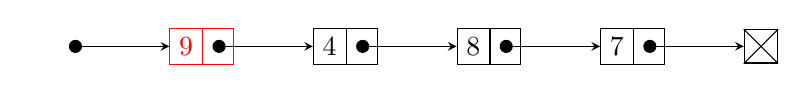
\begin{tikzpicture}[list/.style={rectangle split, rectangle split parts=2, draw, rectangle split horizontal}, >=stealth, start chain]
            \node[list,on chain,white] (a0) {};
            \node[list,on chain,red] (a1) {9};
            \node[list,on chain] (a2) {4};
            \node[list,on chain] (a3) {8};
            \node[list,on chain] (a4) {7};
            \node[on chain,draw,inner sep=6pt] (an) {};
              \draw (an.north east) -- (an.south west);
              \draw (an.north west) -- (an.south east);
            \draw[*->] let \p1 = (a0.two), \p2 = (a0.center) in (\x1,\y2) -- (a1);
            \draw[*->] let \p1 = (a1.two), \p2 = (a1.center) in (\x1,\y2) -- (a2);
            \draw[*->] let \p1 = (a2.two), \p2 = (a2.center) in (\x1,\y2) -- (a3);
            \draw[*->] let \p1 = (a3.two), \p2 = (a3.center) in (\x1,\y2) -- (a4);
            \draw[*->] let \p1 = (a4.two), \p2 = (a4.center) in (\x1,\y2) -- (an);
        \end{tikzpicture}\\
        $B$: 
        \begin{tikzpicture}[list/.style={rectangle split, rectangle split parts=2, draw, rectangle split horizontal}, >=stealth, start chain]
            \node[list,on chain,white] (b0) {};
            \node[list,on chain] (b1) {7};
            \node[list,on chain] (b2) {8};
            \node[list,on chain] (b3) {4};
            \node[list,on chain,red] (b4) {5};
            \node[on chain,draw,inner sep=6pt] (bn) {};
              \draw (bn.north east) -- (an.south west);
              \draw (bn.north west) -- (an.south east);
            \draw[*->] let \p1 = (b0.two), \p2 = (b0.center) in (\x1,\y2) -- (b1);
            \draw[*->] let \p1 = (b1.two), \p2 = (b1.center) in (\x1,\y2) -- (b2);
            \draw[*->] let \p1 = (b2.two), \p2 = (b2.center) in (\x1,\y2) -- (b3);
            \draw[*->] let \p1 = (b3.two), \p2 = (b3.center) in (\x1,\y2) -- (b4);
            \draw[*->] let \p1 = (b4.two), \p2 = (b4.center) in (\x1,\y2) -- (bn);
        \end{tikzpicture}\\
        $\langle a\rangle = (9,4,8,7), \langle b\rangle = (5,4,8,7), i=1, a_i=9, b_i=5$.

        Your procedure should take the heads of $A$ and $B$ as its input, then output $i$, while $i$ is the index mentioned above.
        Both $A$ and $B$ are read-only, you cannot modify them.\\
        In $o(n^2)$ time, $O(1)$ extra space.

\item You are given the heads of two read-only linked list $A$ and $B$. They might contain loop. Please follow the guide and design a procedure to determine whether the shapes of the linked lists are identical.\\
        For example, among the following linked lists, linked list $\beta$ and linked list $\delta$ are identical in shape. You may discover that a linked list contains at most one loop, and if there is one, then the loop must appears at the end. Thus, two linked lists are identical in shape if and only if their "chain parts" and the "loop parts" are of equal size respectively.\\

        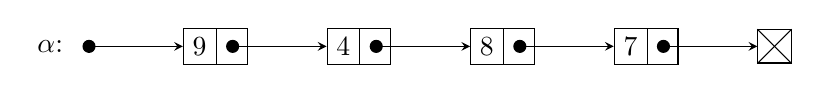
\begin{tikzpicture}[list/.style={rectangle split, rectangle split parts=2, draw, rectangle split horizontal}, >=stealth, start chain]
            \node[list,on chain,draw=white] (a) {$\alpha$: };
            \node[list,on chain] (b) {9};
            \node[list,on chain] (c) {4};
            \node[list,on chain] (d) {8};
            \node[list,on chain] (e) {7};
            \node[on chain,draw,inner sep=6pt] (n) {};
              \draw (n.north east) -- (n.south west);
              \draw (n.north west) -- (n.south east);
            \draw[*->] let \p1 = (a.two), \p2 = (a.center) in (\x1,\y2) -- (b);
            \draw[*->] let \p1 = (b.two), \p2 = (b.center) in (\x1,\y2) -- (c);
            \draw[*->] let \p1 = (c.two), \p2 = (c.center) in (\x1,\y2) -- (d);
            \draw[*->] let \p1 = (d.two), \p2 = (d.center) in (\x1,\y2) -- (e);
            \draw[*->] let \p1 = (e.two), \p2 = (e.center) in (\x1,\y2) -- (n);
        \end{tikzpicture}
        chain part:4, loop part:0\\

        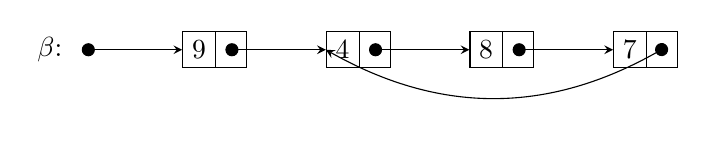
\begin{tikzpicture}[list/.style={rectangle split, rectangle split parts=2, draw, rectangle split horizontal}, >=stealth, start chain]
            \node[list,on chain,draw=white] (a) {$\beta$: };
            \node[list,on chain] (b) {9};
            \node[list,on chain] (c) {4};
            \node[list,on chain] (d) {8};
            \node[list,on chain] (e) {7};
            \draw[*->] let \p1 = (a.two), \p2 = (a.center) in (\x1,\y2) -- (b);
            \draw[*->] let \p1 = (b.two), \p2 = (b.center) in (\x1,\y2) -- (c);
            \draw[*->] let \p1 = (c.two), \p2 = (c.center) in (\x1,\y2) -- (d);
            \draw[*->] let \p1 = (d.two), \p2 = (d.center) in (\x1,\y2) -- (e);
            \path[*->] ($(e.two)+(0.14,0.12)$) edge [bend left] ($(c.west)$);
        \end{tikzpicture}
        chain part:1, loop part:3\\

        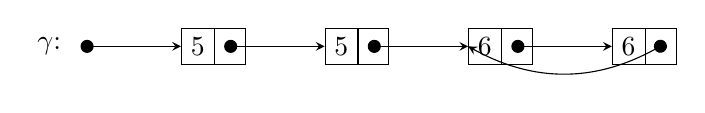
\begin{tikzpicture}[list/.style={rectangle split, rectangle split parts=2, draw, rectangle split horizontal}, >=stealth, start chain]
            \node[list,on chain, draw=white] (a) {$\gamma$: };
            \node[list,on chain] (b) {5};
            \node[list,on chain] (c) {5};
            \node[list,on chain] (d) {6};
            \node[list,on chain] (e) {6};
            \draw[*->] let \p1 = (a.two), \p2 = (a.center) in (\x1,\y2) -- (b);
            \draw[*->] let \p1 = (b.two), \p2 = (b.center) in (\x1,\y2) -- (c);
            \draw[*->] let \p1 = (c.two), \p2 = (c.center) in (\x1,\y2) -- (d);
            \draw[*->] let \p1 = (d.two), \p2 = (d.center) in (\x1,\y2) -- (e);
            \path[*->] ($(e.two)+(0.14,0.12)$) edge [bend left] ($(d.west)$);
        \end{tikzpicture}
        chain part:2, loop part:2\\

        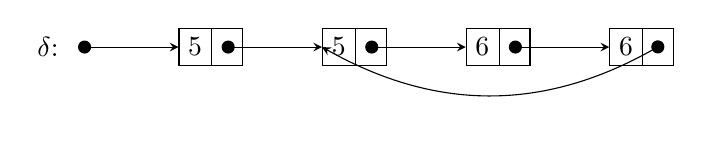
\begin{tikzpicture}[list/.style={rectangle split, rectangle split parts=2, draw, rectangle split horizontal}, >=stealth, start chain]
            \node[list,on chain,draw=white] (a) {$\delta$: };
            \node[list,on chain] (b) {5};
            \node[list,on chain] (c) {5};
            \node[list,on chain] (d) {6};
            \node[list,on chain] (e) {6};
            \draw[*->] let \p1 = (a.two), \p2 = (a.center) in (\x1,\y2) -- (b);
            \draw[*->] let \p1 = (b.two), \p2 = (b.center) in (\x1,\y2) -- (c);
            \draw[*->] let \p1 = (c.two), \p2 = (c.center) in (\x1,\y2) -- (d);
            \draw[*->] let \p1 = (d.two), \p2 = (d.center) in (\x1,\y2) -- (e);
            \path[*->] ($(e.two)+(0.14,0.12)$) edge [bend left] ($(c.west)$);
        \end{tikzpicture}
        chain part:1, loop part:3\\

        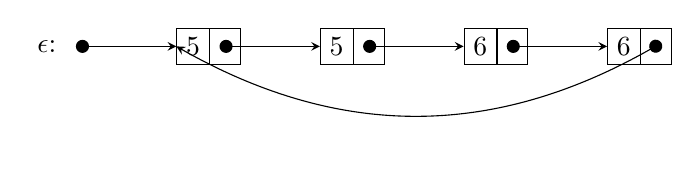
\begin{tikzpicture}[list/.style={rectangle split, rectangle split parts=2, draw, rectangle split horizontal}, >=stealth, start chain]
            \node[list,on chain,draw=white] (a) {$\epsilon$: };
            \node[list,on chain] (b) {5};
            \node[list,on chain] (c) {5};
            \node[list,on chain] (d) {6};
            \node[list,on chain] (e) {6};
            \draw[*->] let \p1 = (a.two), \p2 = (a.center) in (\x1,\y2) -- (b);
            \draw[*->] let \p1 = (b.two), \p2 = (b.center) in (\x1,\y2) -- (c);
            \draw[*->] let \p1 = (c.two), \p2 = (c.center) in (\x1,\y2) -- (d);
            \draw[*->] let \p1 = (d.two), \p2 = (d.center) in (\x1,\y2) -- (e);
            \path[*->] ($(e.two)+(0.14,0.12)$) edge [bend left] ($(b.west)$);
        \end{tikzpicture}
        chain part:0, loop part:4\\

        Both $A$ and $B$ are read-only, you cannot modify them.
    \begin{enumerate}[label=\alph*.]
        \item Please complete the C function below to determine whether the given linked list has a loop. If so, return a pointer to an arbitrary node on the loop.  Otherwise, return \textit{NULL}.\\
        In $O(n)$ time, $O(1)$ extra space, while $n$ is the number of nodes of the given linked list. Please note that the only input is the head of the linked list, and you are ignorant of $n$.

\begin{lstlisting}
typedef struct list_node{
    void* data;
    struct list_node *next;
} list_node;
*list_node isLoop(list_node *head){
    //fill the blank here
}
\end{lstlisting}

        \item Please complete the C function below to determine the length of the loop of the given linked list. The length of the loop is defined as the number of nodes on the loop.\\
        In $O(n)$ time, $O(1)$ extra space.

\begin{lstlisting}
unsigned int loopLength(list_node *head){
    //fill the blank here
}
\end{lstlisting}
\end{enumerate}
        Please describe a procedure that determine whether $A$ and $B$ are of same shape. Your procedure should takes the heads of $A$ and $B$ as its input. If they are of same shape, output $1$, otherwise, output $0$. In:
\begin{enumerate}[label=\alph*.]
    \setcounter{enumii}{2}
        \item $O(n \lg n)$ time, $O(1)$ extra space.
        \item $O(n)$ time, $O(n)$ extra space.\\
    \noindent $n$ is the sum of the numbers of nodes of $A$ and $B$, and you are ignorant of $n$.
    \end{enumerate}

\end{enumerate}
\end{problem}

\newpage

\vspace{5pt}
\begin{center}
\textbf{\large Programming problems}
\end{center}
\begin{problem}Notepad -{}-

You are required to simulate a very lightweight text editor: \textit{Notepad-}-. The following table shows all the effective keys in this editor and their effects. All other keys are ineffective and {\bfseries should be ignored} by the editor.
\begin{table}[h]
\centering
\begin{tabularx}{\textwidth}{|l|X|}
\hline
\texttt{a-z} & Overwrite the selected segment with the character; if nothing is selected, simply write the character. Exit \textit{selection mode}.\\\hline
\texttt{H}   & Move the cursor leftward by one. If the cursor is at the beginning file, do nothing.\\\hline
\texttt{L}   & Move the cursor rightward by one. If the cursor is at the end file, do nothing.\\\hline
\texttt{V}   & Enter \textit{selection mode}.\\\hline
\texttt{D}   & Cut the selected segment and overwrite the clipboard with it. Exit \textit{selection mode}.\\\hline
\texttt{P}   & Overwrite the selected segment with the content in the clipboard; if nothing is selected, simply paste the clipboard content then clear the clipboard. Move the cursor to the end of the pasted content. Exit \textit{selection mode}.\\\hline
\end{tabularx}
\end{table}

Note that the selection mode works just like keeping <shift> key pressed in Notepad or Word. More precisely, in \textit{selection mode}, the "selected segment" is the segment between the current cursor and the cursor position when you enter \textit{selection mode}. While not in selection mode, nothing is selected.\\
Suppose \textit{Arvin} just open an empty file with \textit{Notepad-}-, and the clipboard is initially empty. Given the series of keys pressed by \textit{Arvin}, what would the file eventually be?\\

\textbf{\large Input Format}\\
The first line is an integer $T$, indicating that there are $T$ test cases. For every test cases there is  a string composed of lowercase and uppercase characters, which is the series of keys Arvin keys in.\\

\textbf{\large Output Format}\\
For every test case, output the final content of the file.\\

\textbf{\large Sample Input}\\
\texttt{ 2\\tleVHHHwaVHHac\\dsahahaVHHHHDggHHHHHPLLLLLgggqaq }\\

\textbf{\large Sample Output}\\
\texttt{ac\\hahadsagggggqaq }\\
\end{problem}
\newpage

\begin{problem}The Crafty TA

Given $2$ positive integers $N$, $k$, you can obtain a new integer by removing $k$ digits from $N$. Please output the least one that does not contain any leading zeros.\\

\textbf{\large Input Format}\\
$2$ integers, $N$ and $k$.\\
$1\leq N\leq 10^{10^8}$\\
$1\leq k\leq\min(\log_{10}n, 10^3)$\\

\textbf{\large Output Format}\\
An $(\log_{10}n-k)$-digit number, which is the least number you can obtain by removing $k$ digits from $N$.\\

\textbf{\large Sample Input}\\
\texttt{30400 2}\\

\textbf{\large Sample Output}\\
\texttt{300}\\
\end{problem}

\end{document}
